\documentclass{article}

\usepackage[utf8]{inputenc}
\usepackage[T1]{fontenc}
\usepackage{datetime}
\usepackage{graphicx}
\usepackage{float}
\usepackage{subcaption}

\usepackage{minted}
\usepackage[os=win]{menukeys}
\usepackage{tikz}

\usepackage[english]{babel}
\usepackage{geometry}

\usepackage{adjustbox}
\usepackage{multirow}
\usepackage{hyperref}
\usepackage{titlesec}

\geometry{
	a4paper,
	left=25mm,
	right=25mm,
	top=25mm,
	bottom=25mm,
}

\hypersetup{
	colorlinks=true,
	linkcolor=blue,
	urlcolor=blue,
}

\setcounter{secnumdepth}{4}
\renewcommand{\theparagraph}{\thesubsubsection.\alph{paragraph}}

\addto\captionsenglish{\renewcommand{\contentsname}{Daftar Isi}}
\addto\captionsenglish{\renewcommand{\tablename}{Tabel}}
\addto\captionsenglish{\renewcommand{\figurename}{Gambar}}
\addto\captionsenglish{\renewcommand{\refname}{}}

\def\mydate{\leavevmode\hbox{\the\year-\twodigits\month-\twodigits\day}}
\def\twodigits#1{\ifnum#1<10 0\fi\the#1}

% this custom commands below will not work if not run on GNU/Linux
\newcommand{\ShowOsVersion}{
	\immediate\write18{\unexpanded{foo=`uname -srom | tr '_' '-'` && echo -n "${foo}" > tmp.txt}}
	\unskip\unskip\input{tmp.txt}\unskip
	\immediate\write18{rm tmp.txt}
}
\newcommand{\ShowTexVersion}{
	\immediate\write18{\unexpanded{foo=`pdflatex -version | head -n1 | cut -d' ' -f1,2` && echo -n "${foo}" > tmp.txt}}
	\unskip\unskip\input{tmp.txt}\unskip
	\immediate\write18{rm tmp.txt}
}

\begin{document}
\begin{titlepage}
		\centering

		{
			\LARGE
			\bf
			Laporan Kegiatan Kalibrasi Simulator Telinga
		}

		\bigskip

		{
			\large
			\bf
			Tim Penelitian Audiometer Portable Elbicare
		}

		\vfill

		\begin{figure}[H]
			\centering
			
\includegraphics[width=250pt,angle=0]{images/elbicare-logo}
		\end{figure}

		\vfill

        \bigskip

        {
            \bf
            Achmadi ST MT dan M. Ammar Asyraf ST MT
        }
	\end{titlepage}

	\newpage

	\textbf{Tentang Dokumen}\\

	\noindent Dokumen ini ditulis menggunakan {\textbf{\ShowTexVersion}}pada sistem operasi {\textbf{\ShowOsVersion}}yang
	diupdate terakhir pada tanggal {\mydate} di jam \currenttime.\\

	Kode sumber dokumen ini dapat ditemukan di laman repositori proyek
	\url{https://github.com/VibrasticLab/pikoakustik2/tree/master/prototrial/dokumen/berita_acara/itb_july2023/test_calib}.

	\newpage

	\tableofcontents

	\newpage
	\section{Pendahuluan}

	Dokumen ini adalah rangkuman kegiatan kalibrasi perangkat simulator telinga menggunakan metode ruang dengung.

	\subsection{Tujuan Kegiatan}

	Tujuan utama kegiatan ini adalah mendapatkan rekaman derau yang dapat digunakan sebagai input acuan kalibrasi
	dari setiap unit simulator telinga dimana besar rekaman derau tersebut dibandingkan dengan Sound Level Meter terkalibrasi.

	\subsection{Waktu dan Tempat}

	Kegiatan ini dilakukan di Ruang Dengung dan Ruang Kedap Gedung Adhiwijogo di Institut Teknologi Bandung pada tanggal 7 Juli 2023.

	\subsection{Alat dan Perlengkapan}

	Alat yang digunakan meliputi:

	\begin{itemize}
		\item Speaker merek Yamaha dengan Amplifier board portabel.

		\begin{figure}[H]
			\centering
			\begin{subfigure}[]{.45\textwidth}
				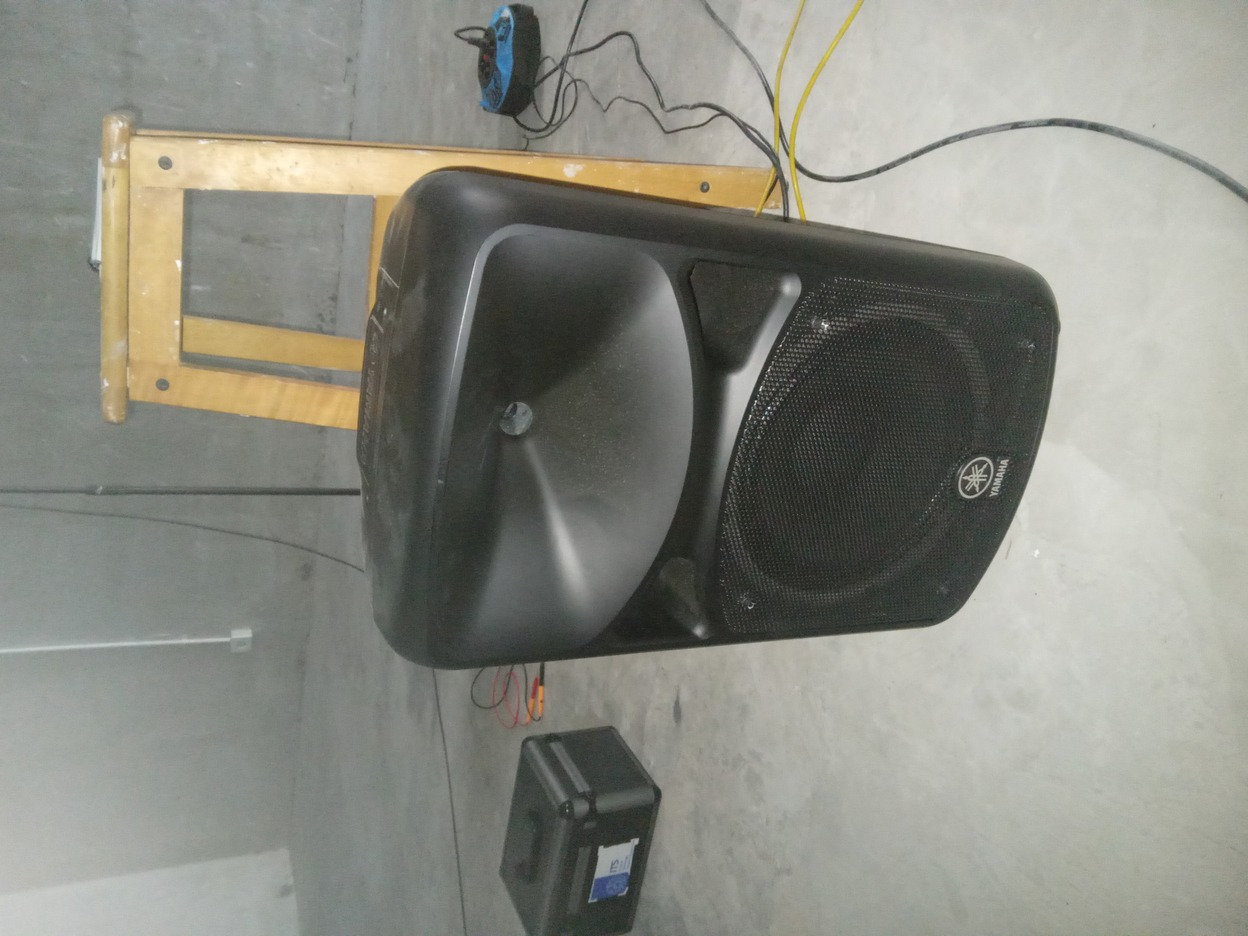
\includegraphics[width=\textwidth,angle=-90]{images/tools_speaker}
				\caption{Speaker}
			\end{subfigure}
			\begin{subfigure}[]{.45\textwidth}
				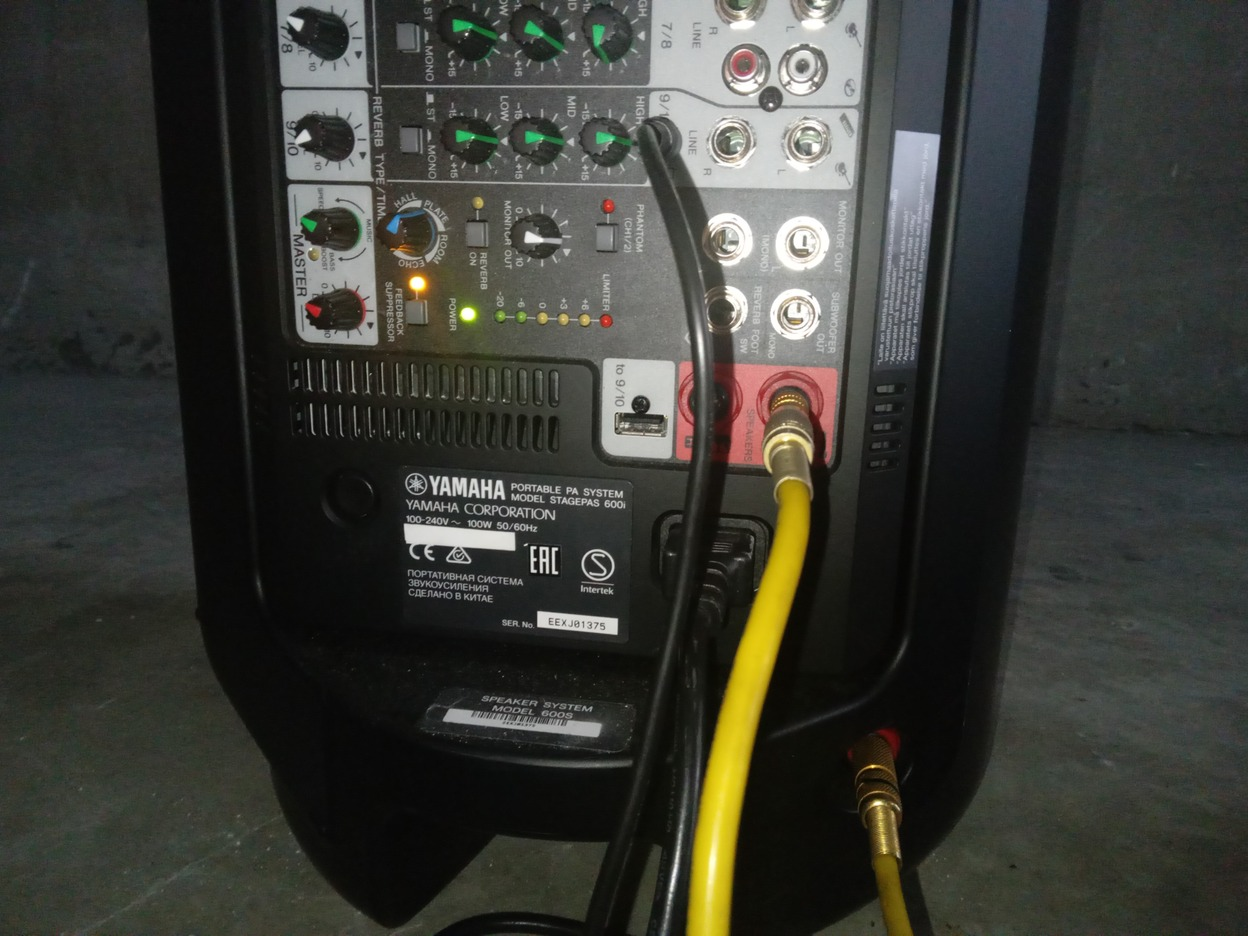
\includegraphics[width=\textwidth]{images/tools_amplifier}
				\caption{Amplifier}
			\end{subfigure}
			\caption{Perangkat Speaker}
		\end{figure}

		\item Sound Level Meter Merek Rion yang telah terkalibrasi.

		\begin{figure}[H]
			\centering
			\begin{subfigure}[]{.35\textwidth}
				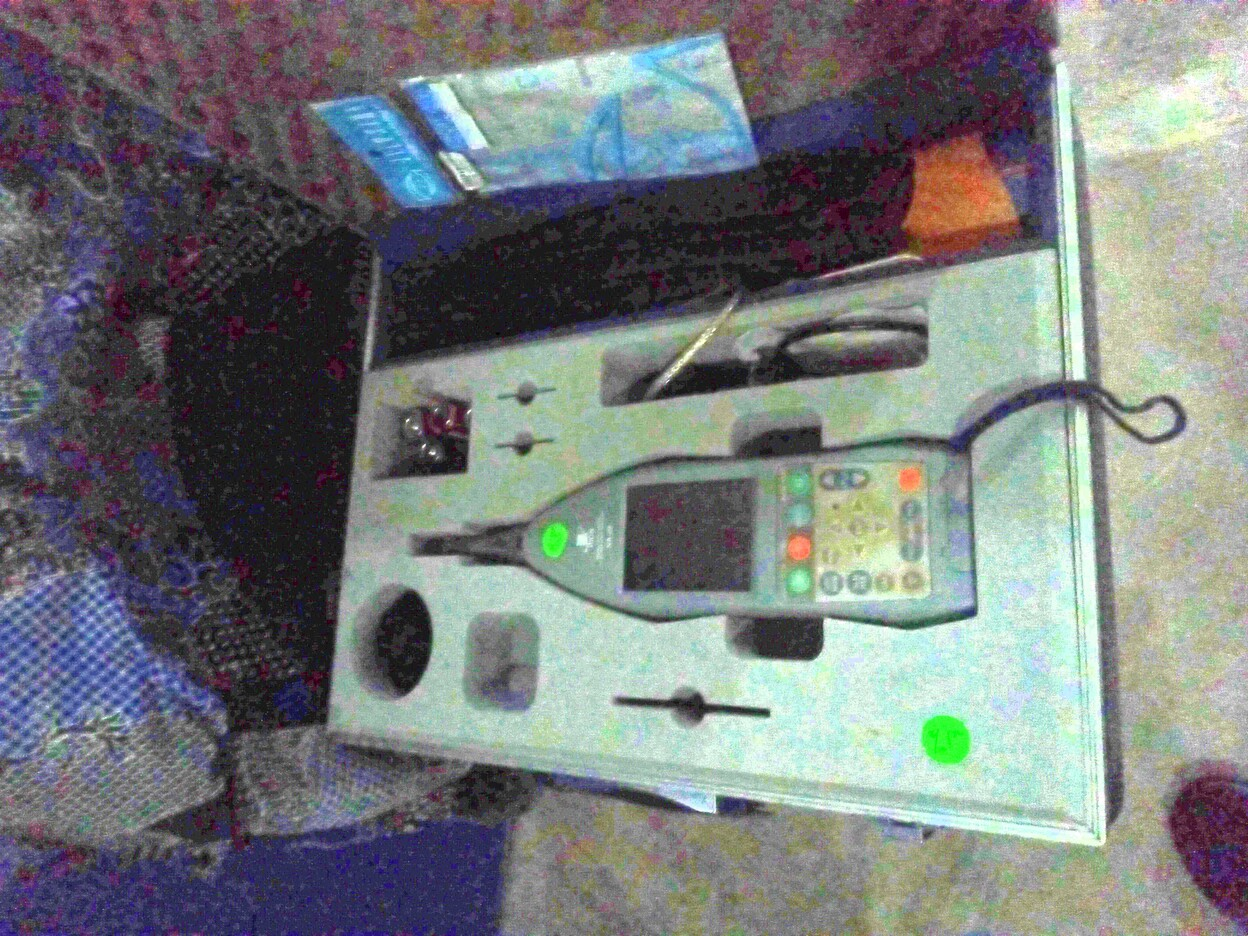
\includegraphics[width=\textwidth]{images/tools_slm_box}
				\caption{SLM RION}
			\end{subfigure}
			\begin{subfigure}[]{.25\textwidth}
				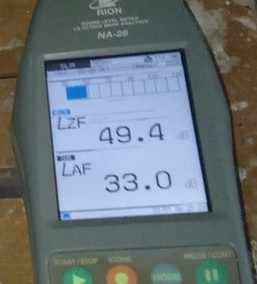
\includegraphics[width=\textwidth]{images/tools_lowest}
				\caption{Noise paling rendah}
			\end{subfigure}
			\caption{Perangkat SLM}
		\end{figure}

		\item Unit MiniDSP EARS sebagai Simulator Telinga. Ini adalah unit simulator telinga pertama.
		Berikut laman produk: \href{https://www.minidsp.com/products/acoustic-measurement/ears-headphone-jig}{MiniDSP EARS}

		\begin{figure}[H]
			\centering
			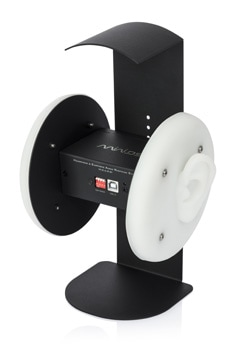
\includegraphics[width=100pt,angle=0]{images/ears}
			\caption{Unit MiniDSP EARS}
		\end{figure}

		\item Unit Microphone 3DIO dan AudioBox Presonus USB96. Ini adalah unit simulator telinga kedua.
		Berikut laman produk: \href{https://3diosound.com/products/free-space-pro-binaural-microphone}{3DIO}
		dan \href{https://www.frontendaudio.com/presonus-audiobox-usb-96-usb-audio-interface/}{AudioBox USB96}

		\begin{figure}[H]
			\centering
			\begin{subfigure}[]{.40\textwidth}
				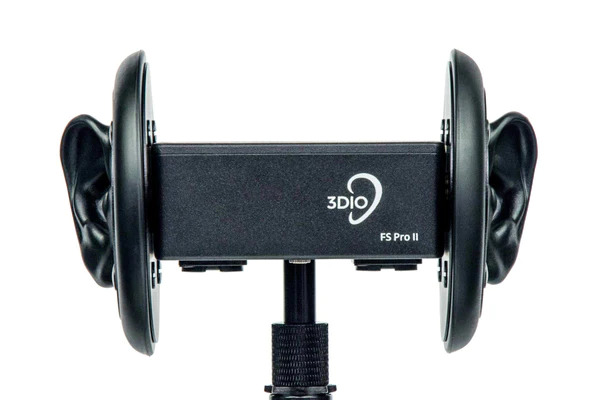
\includegraphics[width=\textwidth]{images/3dio}
				\caption{Microphone 3DIO}
			\end{subfigure}
			\begin{subfigure}[]{.40\textwidth}
				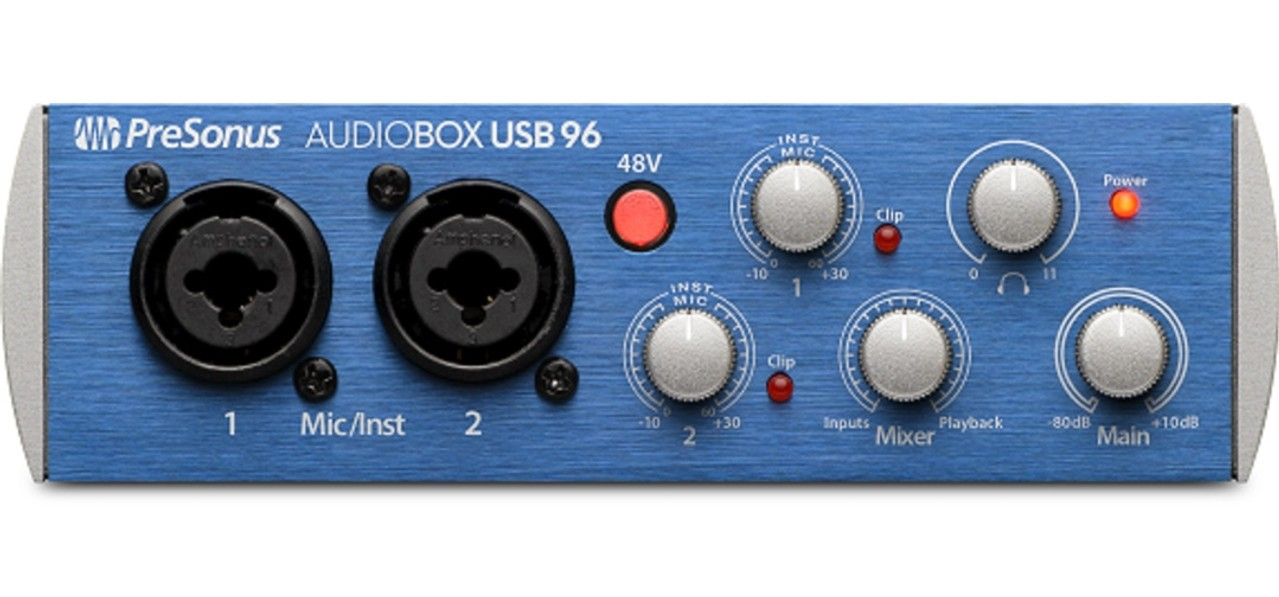
\includegraphics[width=\textwidth]{images/audiobox}
				\caption{Audiobox USB96}
			\end{subfigure}
			\caption{Perangkat 3DIO}
		\end{figure}
	
		\item Perangkat KEMAR buatan GRAS.
		Laman produk: \href{https://www.grasacoustics.com/products/head-torso-simulators-kemar/product/733-45bb}{KEMAR}
		
		\begin{figure}[H]
			\centering
			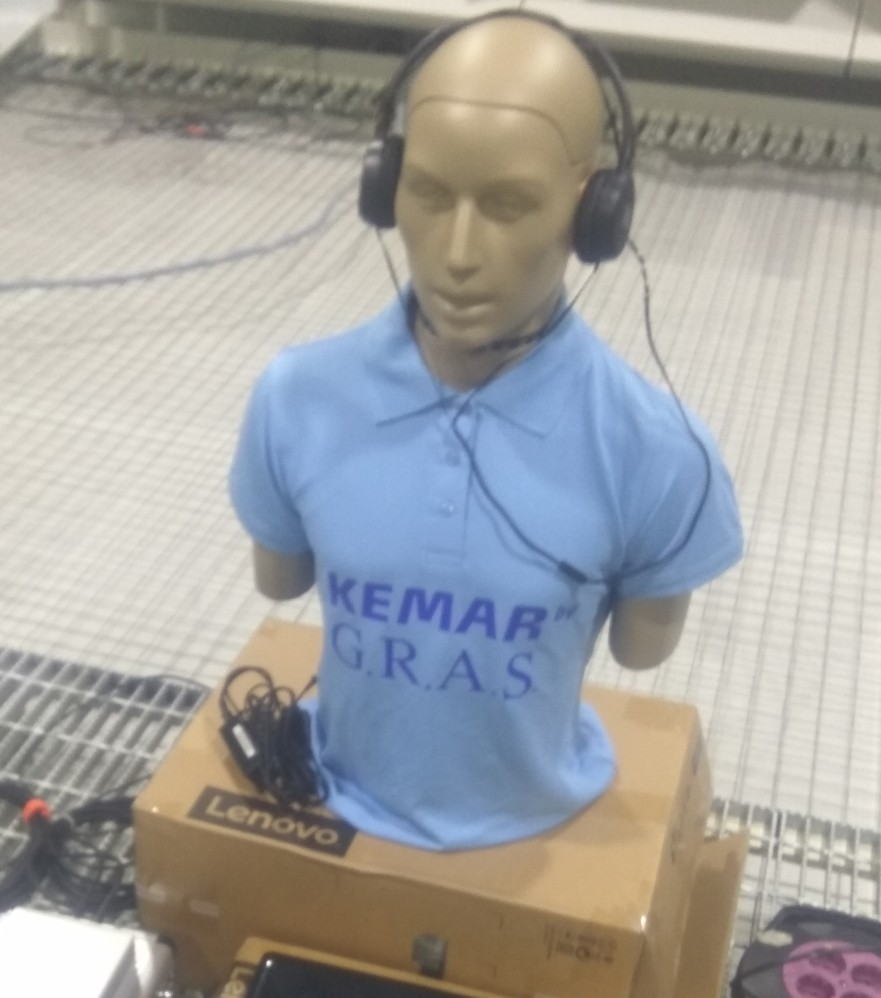
\includegraphics[width=0.35\textwidth,angle=0]{images/kemar}
			\caption{Perangkat KEMAR}
		\end{figure}

		\newpage
		\item Perangkat Lunak Audacity dan RealTime Analyzer dari Yoshimasa.
		Berikut laman produk: \href{https://www.audacityteam.org/}{Audacity} dan \href{http://www.ymec.com/products/dssf3e/}{RTA}.

		\begin{figure}[H]
			\centering
			\begin{subfigure}[]{.55\textwidth}
				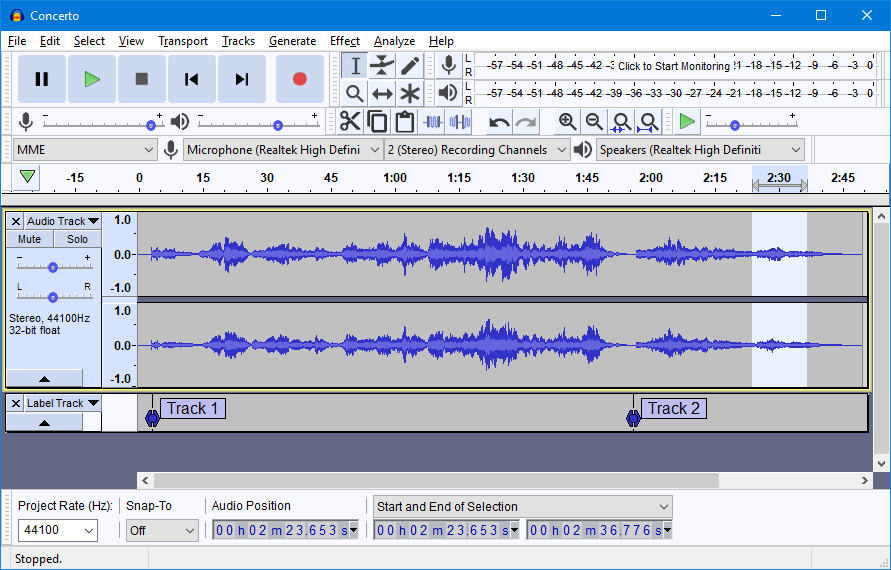
\includegraphics[width=\textwidth]{images/audacity}
				\caption{Audacity}
			\end{subfigure}
			\\
			\begin{subfigure}[]{.55\textwidth}
				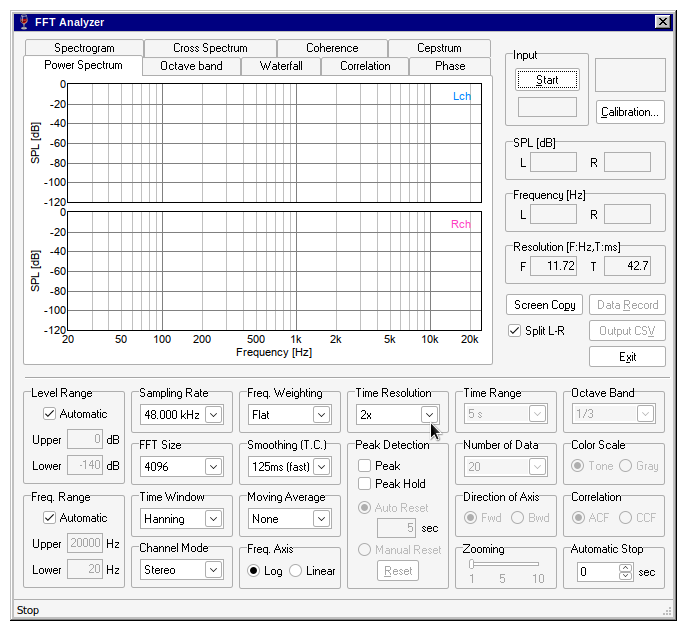
\includegraphics[width=\textwidth]{images/rta}
				\caption{Realtime Analyzer}
			\end{subfigure}
			\caption{Perangkat Lunak}
		\end{figure}

	\end{itemize}

	\newpage
	\section{Kegiatan Kalibrasi}

	\subsection{Unit EARS}

	Berikut rangkuman kegiatan kalibrasi untuk unit MiniDSP EARS.

	\subsubsection{Setup}

	Berikut setup kalibrasi:

	\begin{figure}[H]
		\centering
		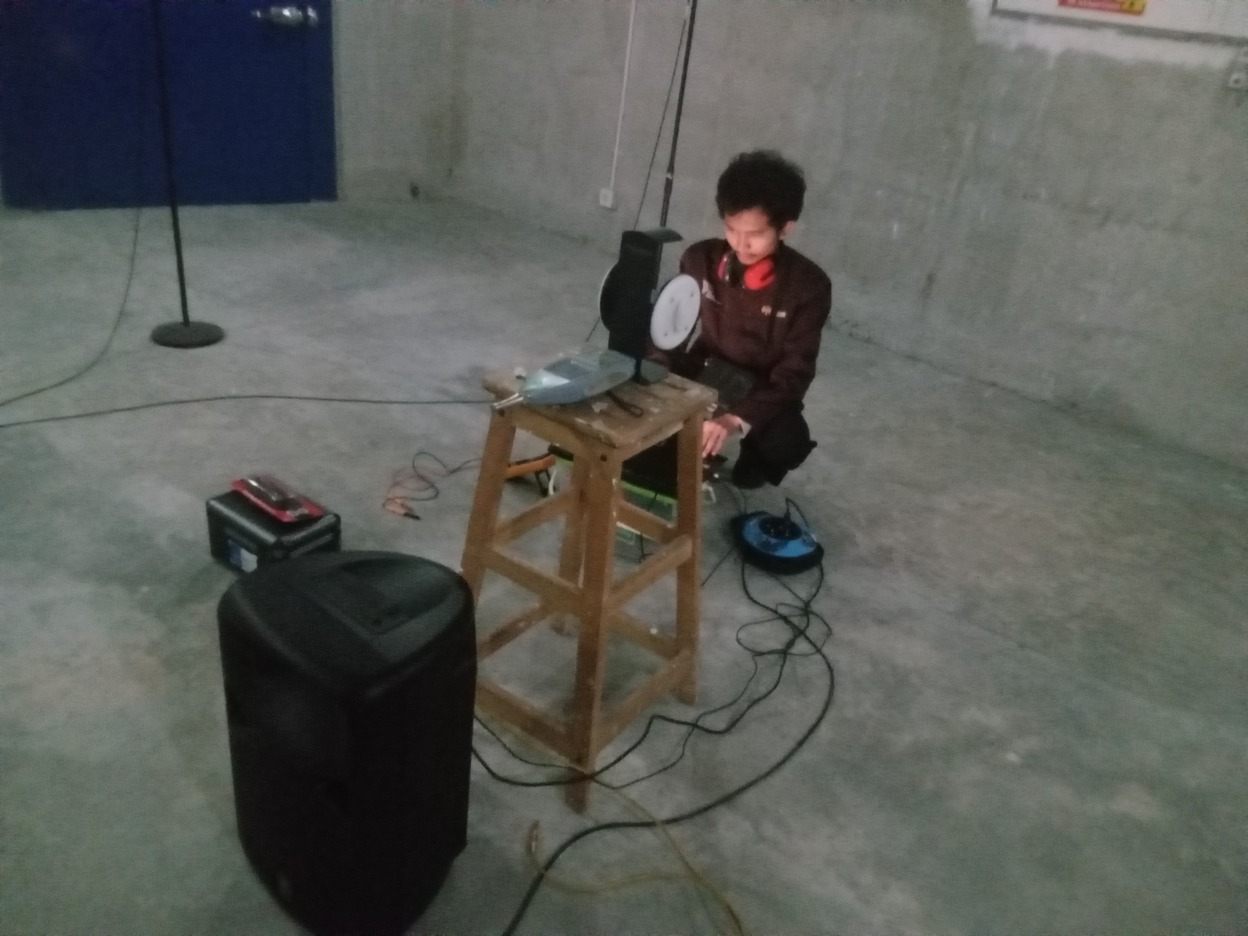
\includegraphics[width=0.8\textwidth,angle=0]{images/ears_setup}
		\caption{Setup posisi EARS, SLM, dan Speaker}
	\end{figure}

	Disini diatur gain pada 0-1-1-1 sebelum sambungan USB ke Laptop.

	\begin{figure}[H]
		\centering
		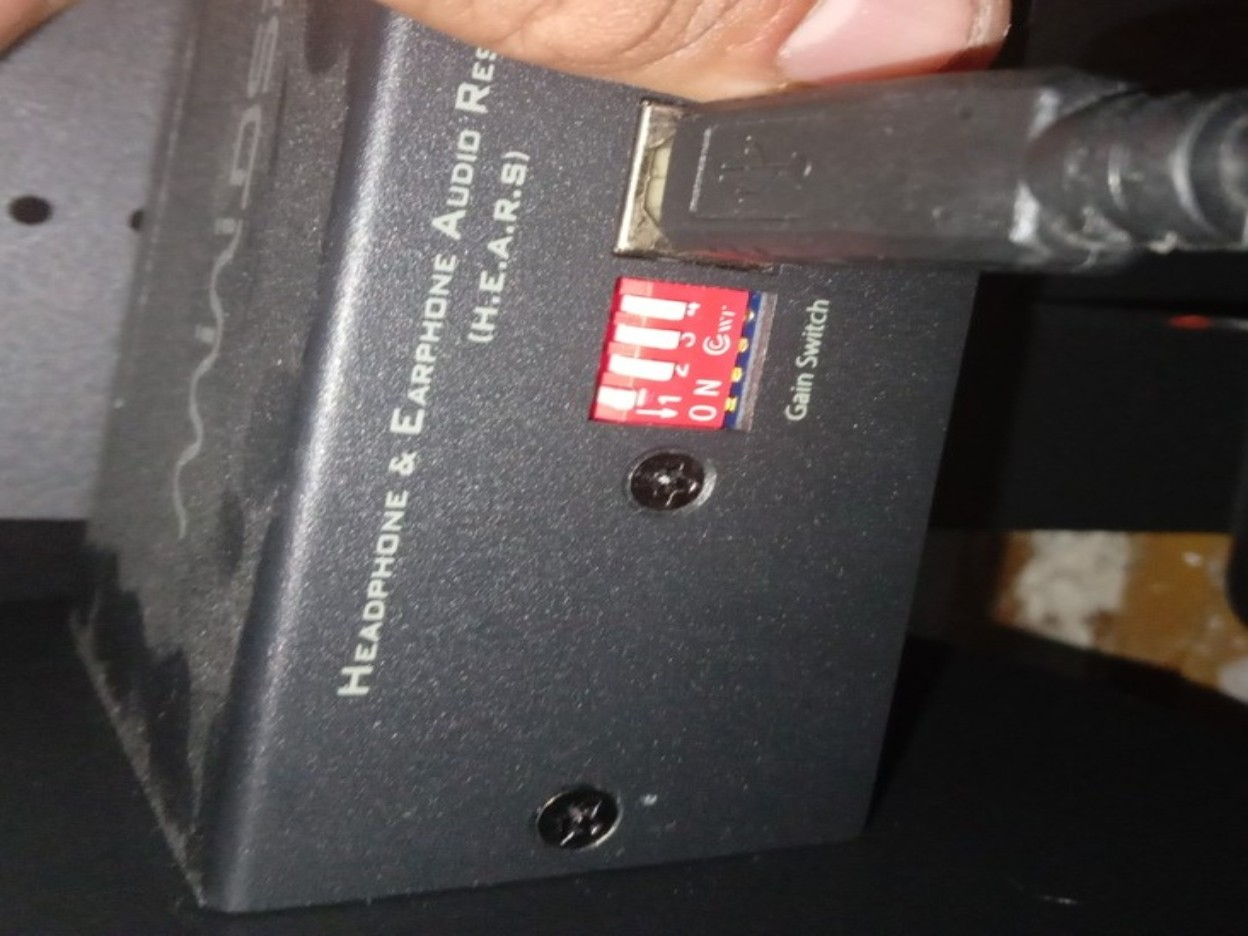
\includegraphics[width=0.5\textwidth,angle=-90]{images/ears_gain}
		\caption{Pengaturan Gain}
	\end{figure}

	\subsubsection{Recording}

	Berikut langkah perekaman noise sebagai acuan kalibrasi:

	\begin{itemize}
		\item Setup perekaman, kemudian sambungkan:
		\begin{itemize}
			\item Kabel USB MiniDSP EARS dan Laptop
			\item Kabel 3.5mm Audio dari Laptop ke Amplifier/Speaker
		\end{itemize}
	
		\item Jalankan Audacity dan pilih input di jendela "Audio Settings".
		Pastikan Input adalah "E.A.R.S Gain: 18dB"
		
		\begin{figure}[H]
			\centering
			\begin{subfigure}[]{.55\textwidth}
				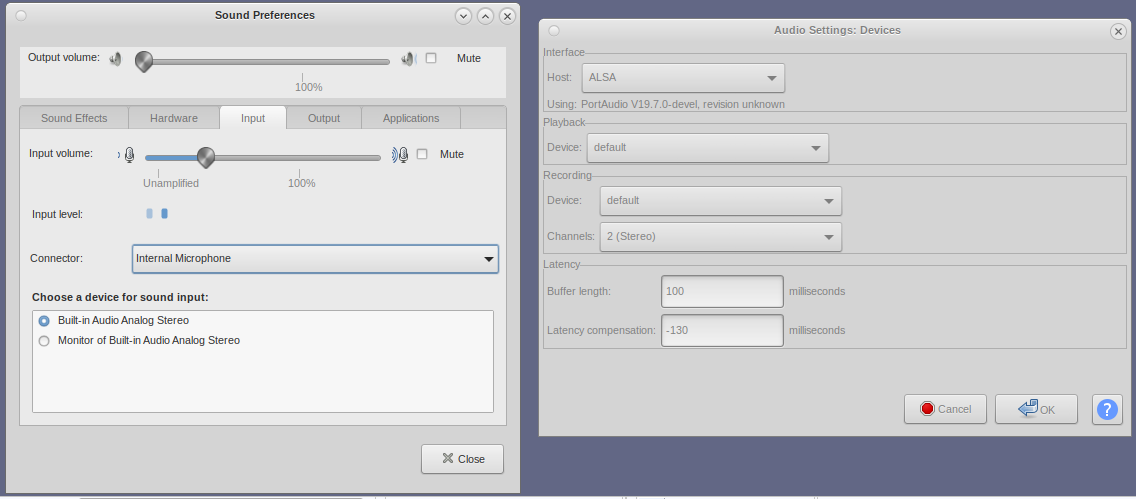
\includegraphics[width=\textwidth]{images/audacity_in_linux}
				\caption{ALSA/PulseAudio di GNU/Linux}
			\end{subfigure}
			\begin{subfigure}[]{.35\textwidth}
				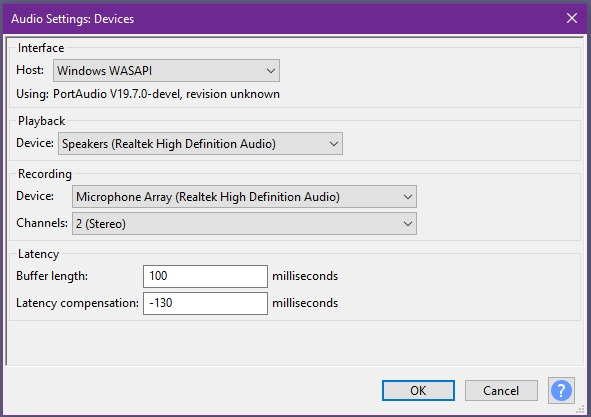
\includegraphics[width=\textwidth]{images/audacity_in_windows}
				\caption{WASAPI di Windows}
			\end{subfigure}
			\caption{Audio Input}
		\end{figure}
		
		\item Jalankan Real-Time Analyzer dan jalankan Signal Generator.
		Pilih White Noise pada volume penuh. Klik Start.
		
		\begin{figure}[H]
			\centering
			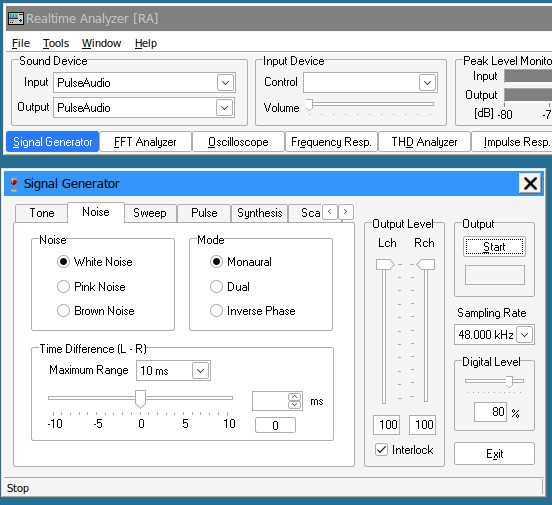
\includegraphics[width=0.6\textwidth,angle=0]{images/rta_noise_gen}
			\caption{Menghasilkan noise}
		\end{figure}
	
		\item Atur Amplifier hingga baca stabil pada nilai tertentu (semisal 80 dB-SPL) pada Sound Level Meter.
		Kemudian rekam noise ruangan di Audacity.
		
		\begin{figure}[H]
			\centering
			\begin{subfigure}[]{.8\textwidth}
				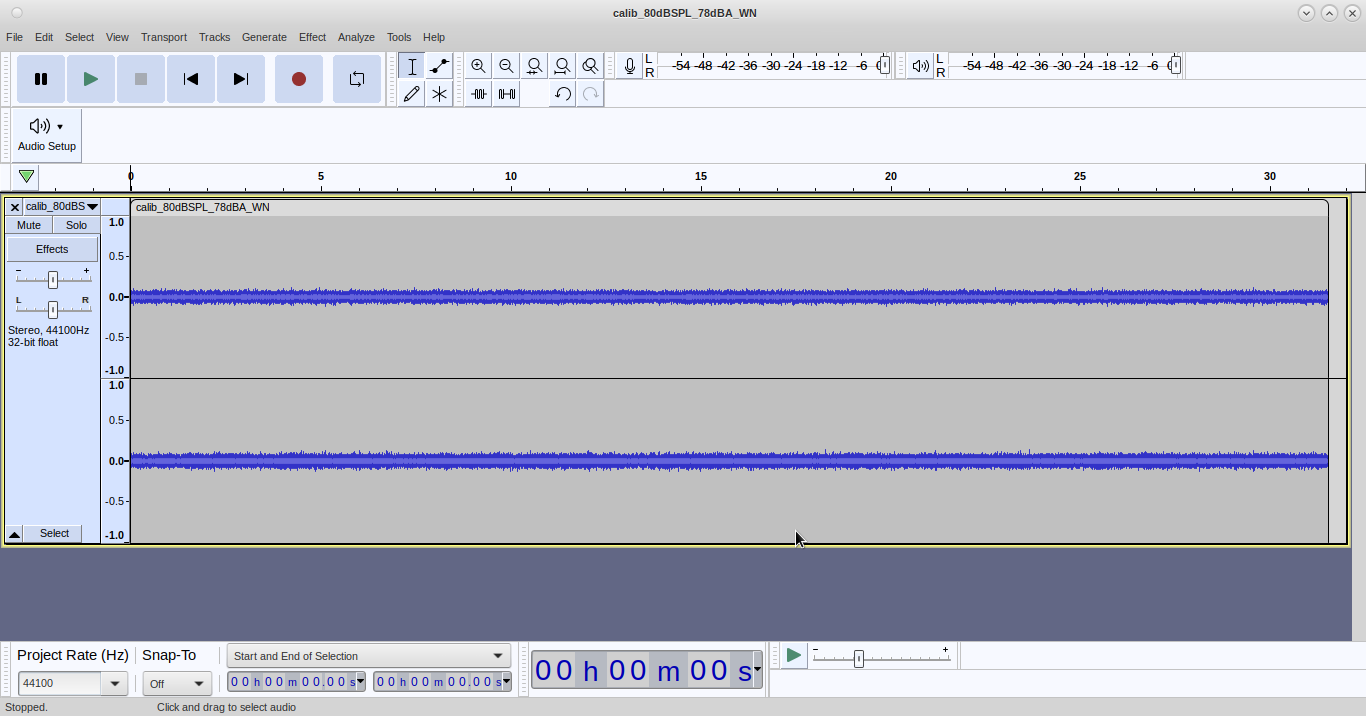
\includegraphics[width=\textwidth]{images/audacity_record}
				\caption{Perekaman di Audacity}
			\end{subfigure}
			\\
			\begin{subfigure}[]{.5\textwidth}
				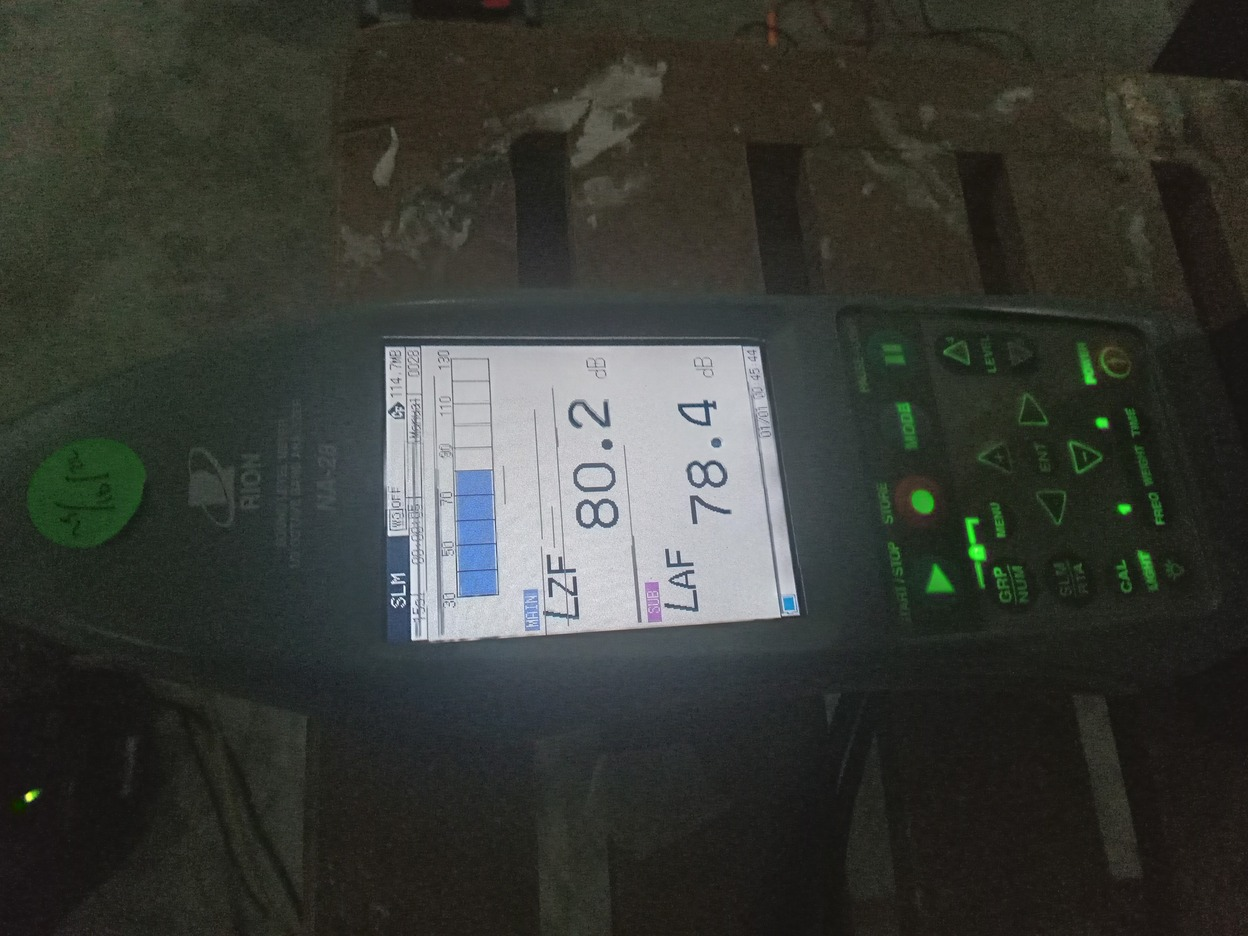
\includegraphics[width=\textwidth]{images/ears_slm_whitenoise}
				\caption{Nilai terbaca pada SLM}
			\end{subfigure}
			\caption{Perekaman Noise}
		\end{figure}
		
		\item Simpan rekaman dalam format WAV.
		Nama file rekaman memiliki informasi nilai pembacaan SLM.
		
		\item Ulangi langkah di atas untuk Pink Noise.
		
		\begin{figure}[H]
			\centering
			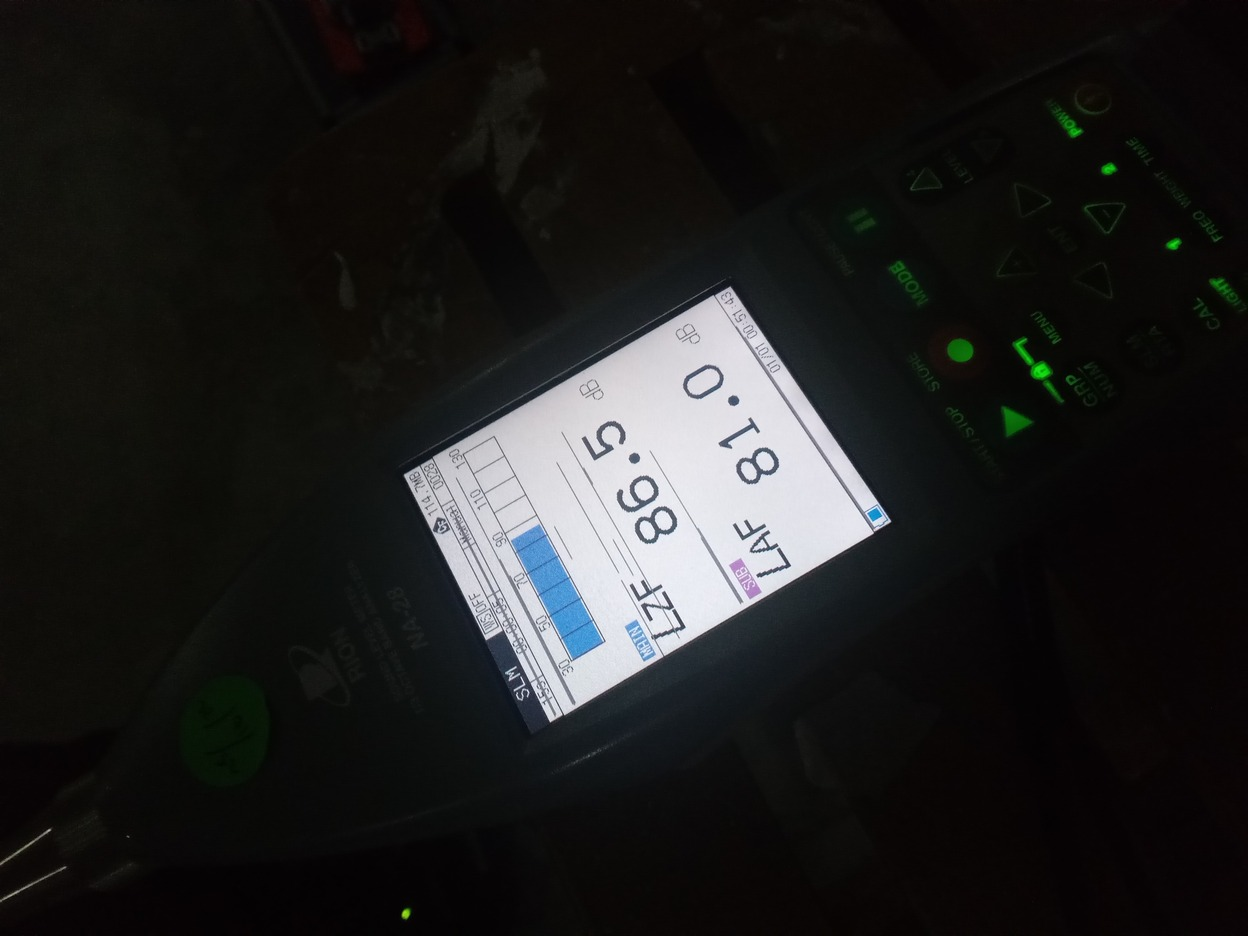
\includegraphics[width=0.5\textwidth,angle=0]{images/ears_slm_pinknoise}
			\caption{Pembacaan Pink Noise}
		\end{figure}
		
	\end{itemize}

	\subsubsection{Kalibrasi}
	
	Untuk kalibrasi, berikut langkah yang dapat dilakukan:
	
	\begin{itemize}
		\item Jalankan Real-Time Analyzer dan buka tab Recorder.
		Pastikan Input adalah PulseAudio (untuk GNU/Linux) atau langsung E.A.R.S (Untuk Windows).
		Kemudian Load rekaman.
		
		\begin{figure}[H]
			\centering
			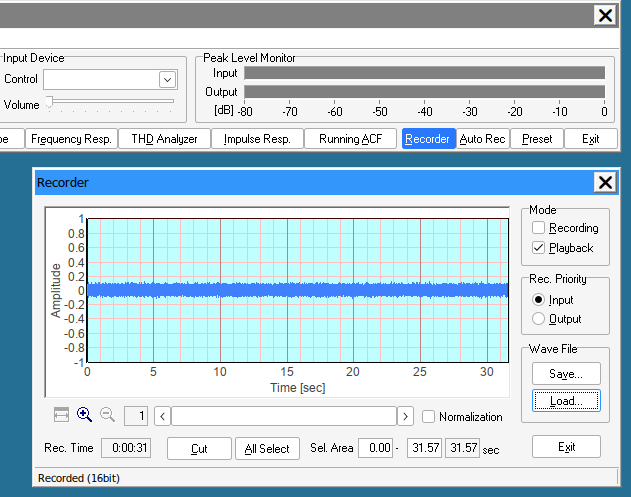
\includegraphics[width=0.6\textwidth,angle=0]{images/rta_load}
			\caption{Loading rekaman ke RTA}
		\end{figure}
	
		Biarkan tab rekaman terbuka.
	
		\item Buka tab FFT Analyzer dan Tekan Calibrate.
		Pilih mode Separate dan atur setiap slider ke nilai 80 dB-SPL sesuai yang terbaca SLM.
		
		\begin{figure}[H]
			\centering
			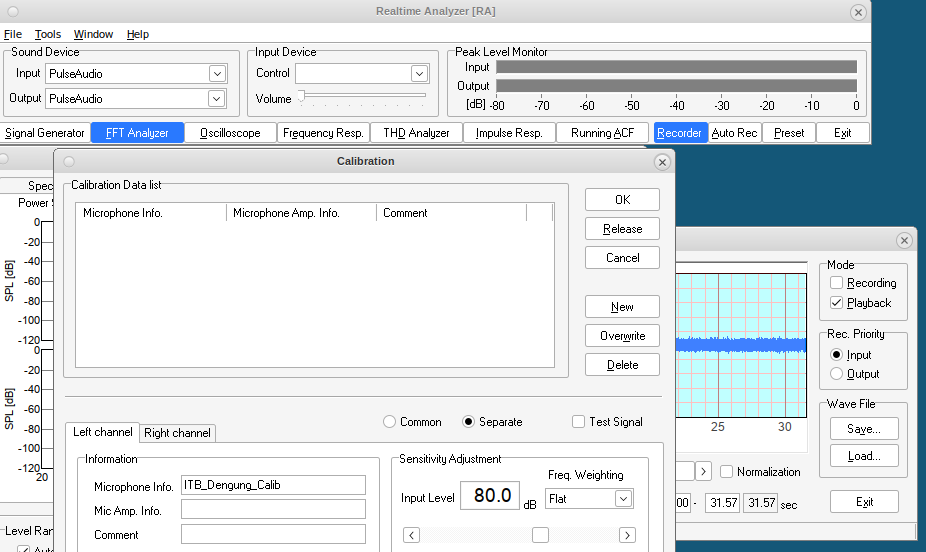
\includegraphics[width=0.8\textwidth,angle=0]{images/rta_calib}
			\caption{Kalibrasi FFT Analyzer}
		\end{figure}
	
		\item Tutup jendela Recorder dan FFT Analyzer terkalibrasi.
		
		\begin{figure}[H]
			\centering
			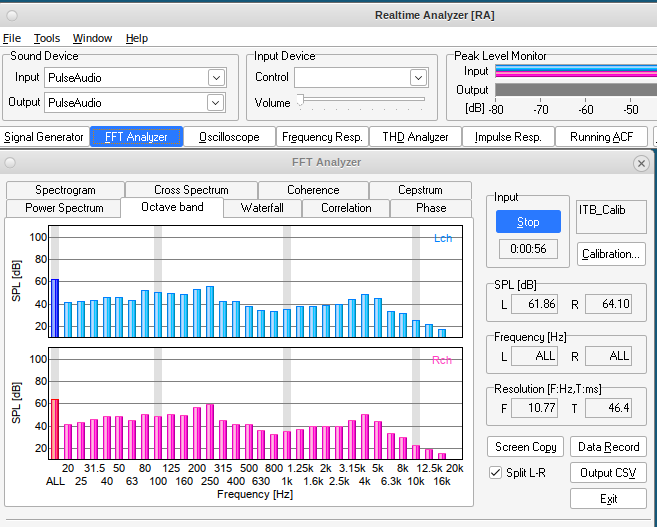
\includegraphics[width=0.8\textwidth,angle=0]{images/rta_fft}
			\caption{Kalibrasi selesai}
		\end{figure}
		
	\end{itemize}

	\newpage
	
	\subsection{Unit 3DIO}
	
	Berikut rangkuman kegiatan kalibrasi untuk unit Microphone 3DIO.

	\subsubsection{Setup}
	
	Berikut setup kalibrasi:
	
	\begin{figure}[H]
		\centering
		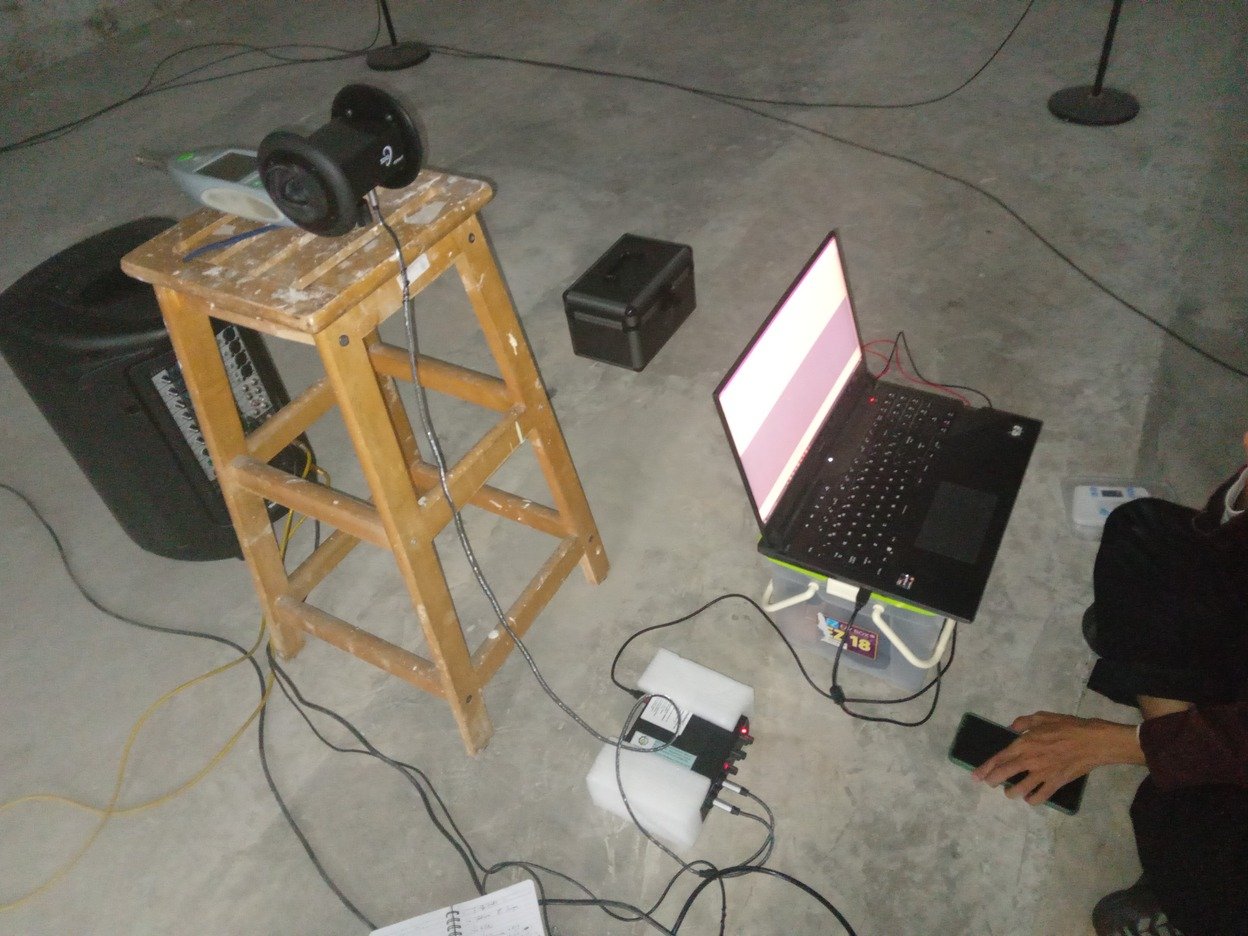
\includegraphics[width=0.75\textwidth,angle=0]{images/3dio_setup}
		\caption{Setup posisi 3DIO, AudioBox, SLM, dan Speaker}
	\end{figure}

	Kemudian sambungkan Mic 3DIO dan AudioBox dengan gain AudioBox di pertengahan:
	
	\begin{figure}[H]
		\centering
		\begin{subfigure}[]{.4\textwidth}
			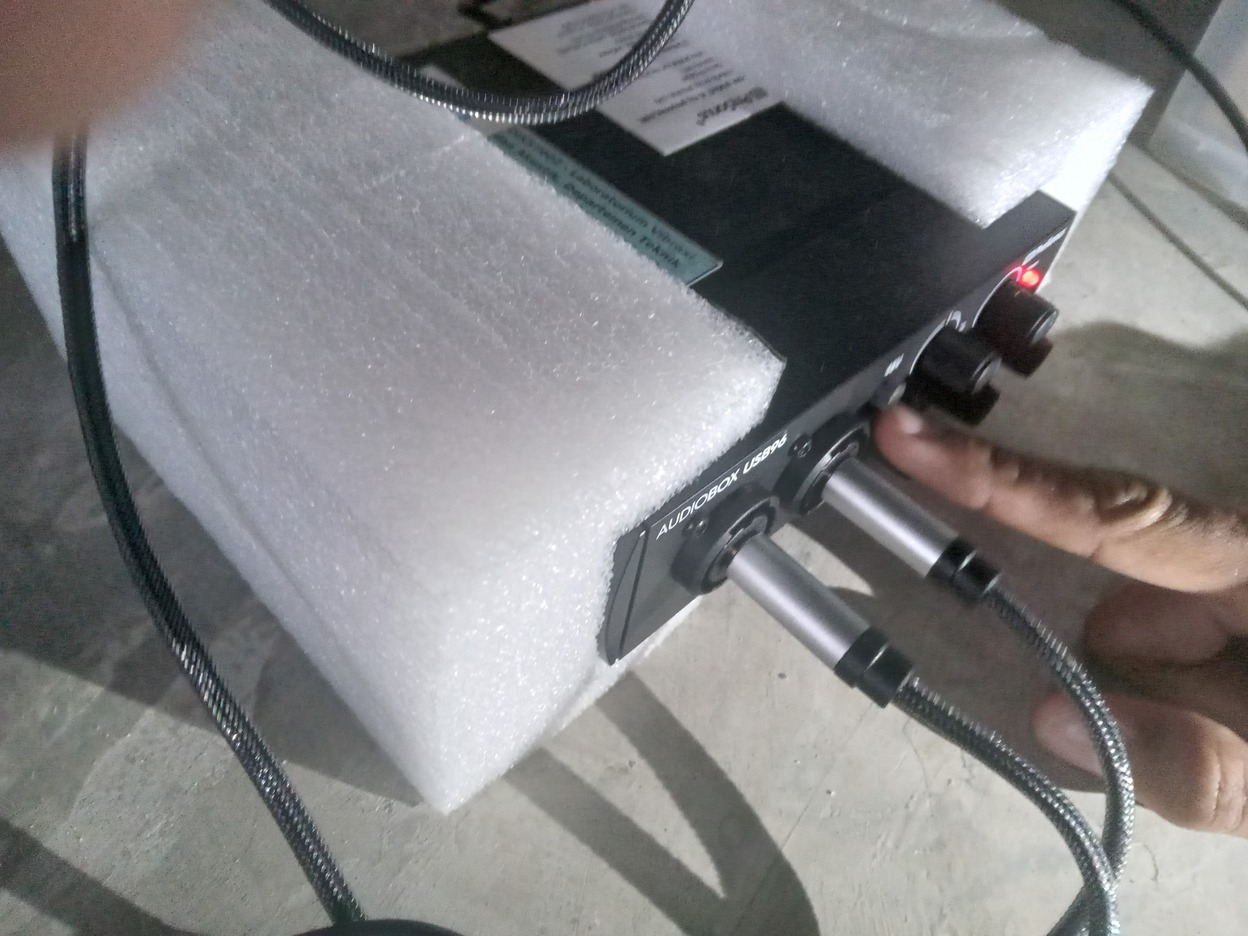
\includegraphics[width=\textwidth]{images/3dio_presonus_jack}
			\caption{Sambungan Audio Jack}
		\end{subfigure}
		\begin{subfigure}[]{.4\textwidth}
			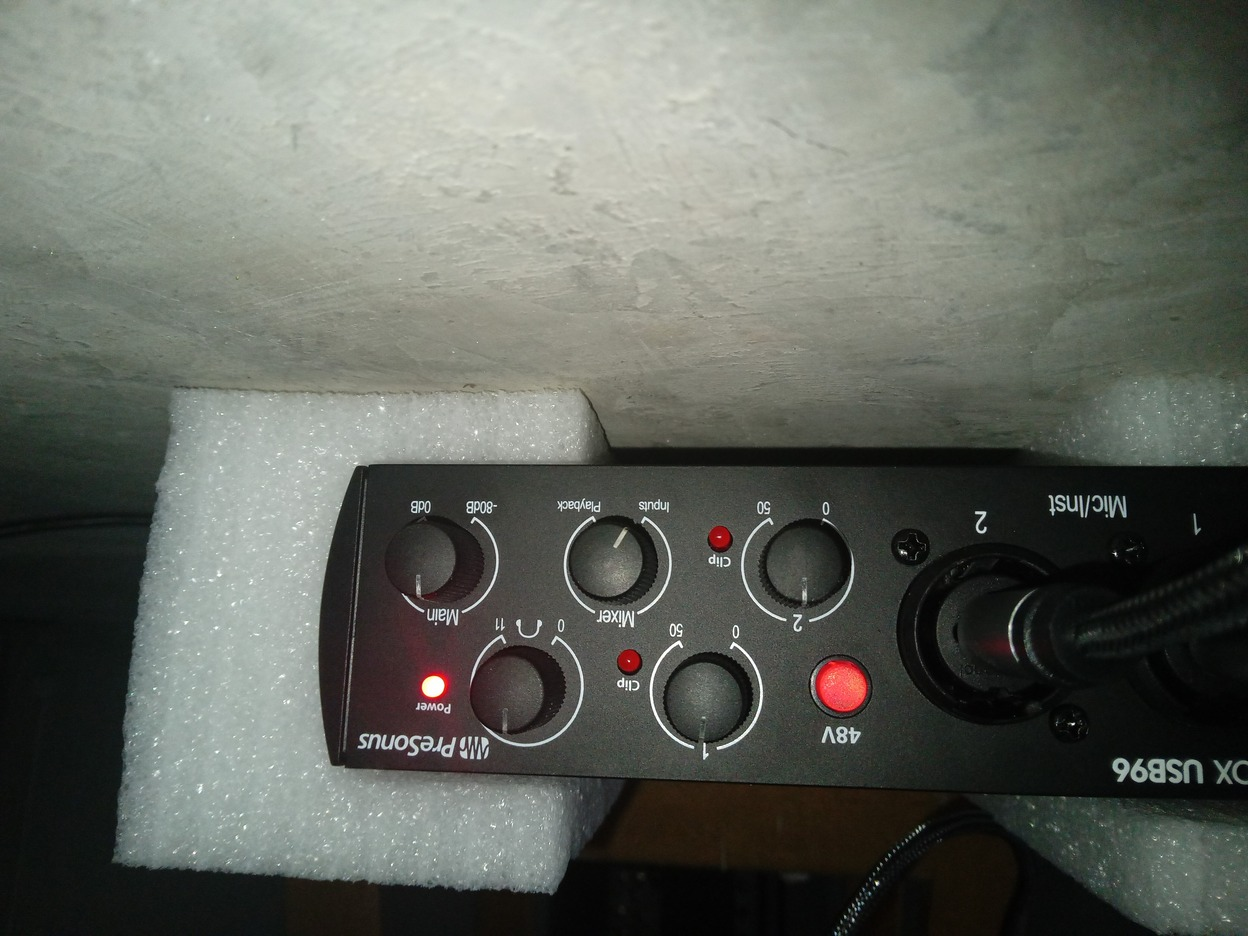
\includegraphics[width=\textwidth,angle=180]{images/3dio_presonus_set}
			\caption{Nilai Gain AudioBox}
		\end{subfigure}
		\\
		\begin{subfigure}[]{.4\textwidth}
			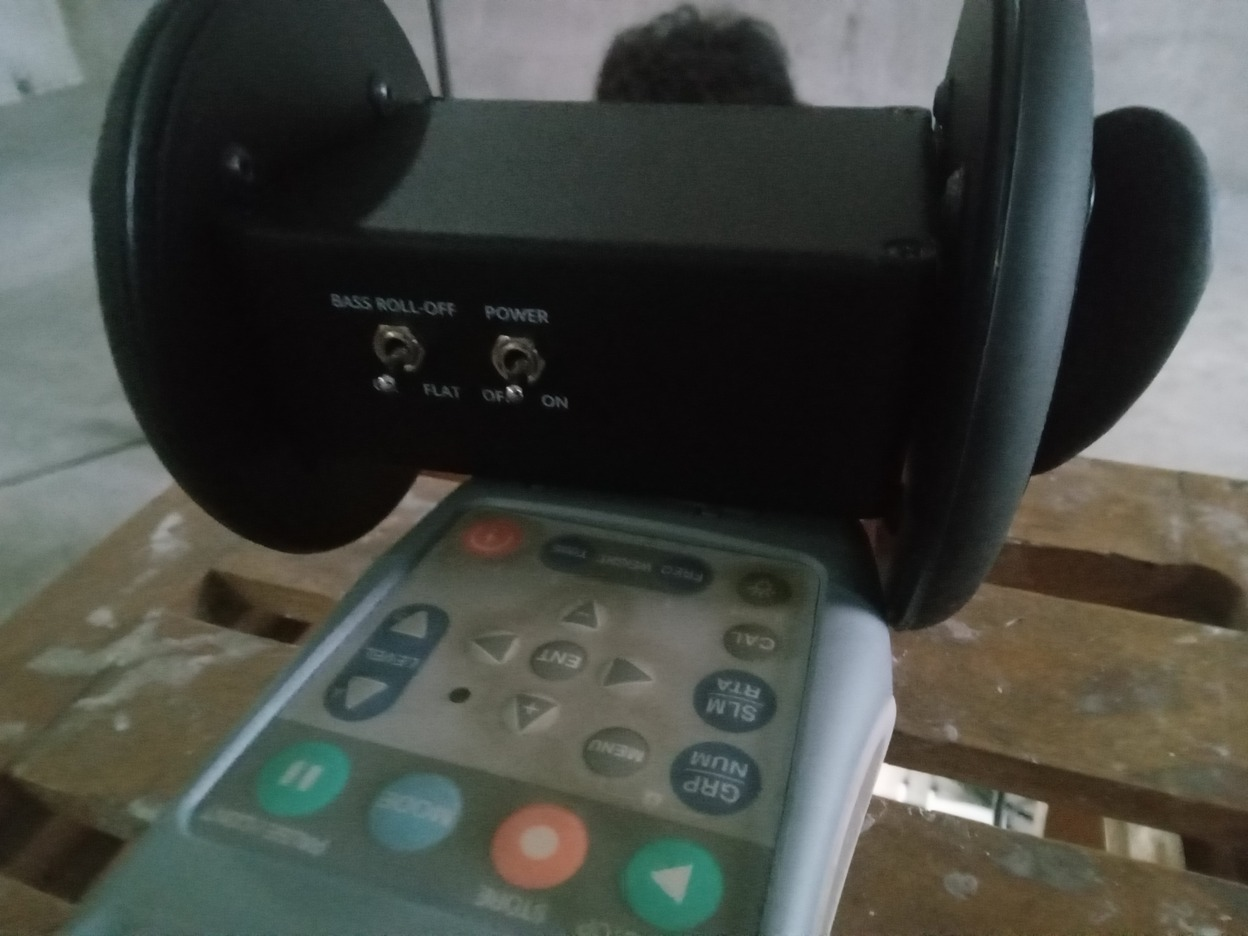
\includegraphics[width=\textwidth,angle=0]{images/3dio_unit_on}
			\caption{Nyalakan 3DIO tanpa Bass-Roll}
		\end{subfigure}
		\caption{Setup AudioBox}
	\end{figure}

	\subsubsection{Recording}
	
	Berikut langkah perekaman noise yang kurang lebih sama dengan unit EARS sebelumnya:
	
	\begin{itemize}
		\item Setup perekaman, kemudian sambungkan:
		\begin{itemize}
			\item Kabel USB AudioBox dan Laptop
			\item Kabel 3.5mm Audio dari Laptop ke Amplifier/Speaker
		\end{itemize}
	
		\item Jalankan Audacity dan pilih input di jendela "Audio Settings".
		Pastikan Input adalah "AudioBox USB96"
		
		\begin{figure}[H]
			\centering
			\begin{subfigure}[]{.55\textwidth}
				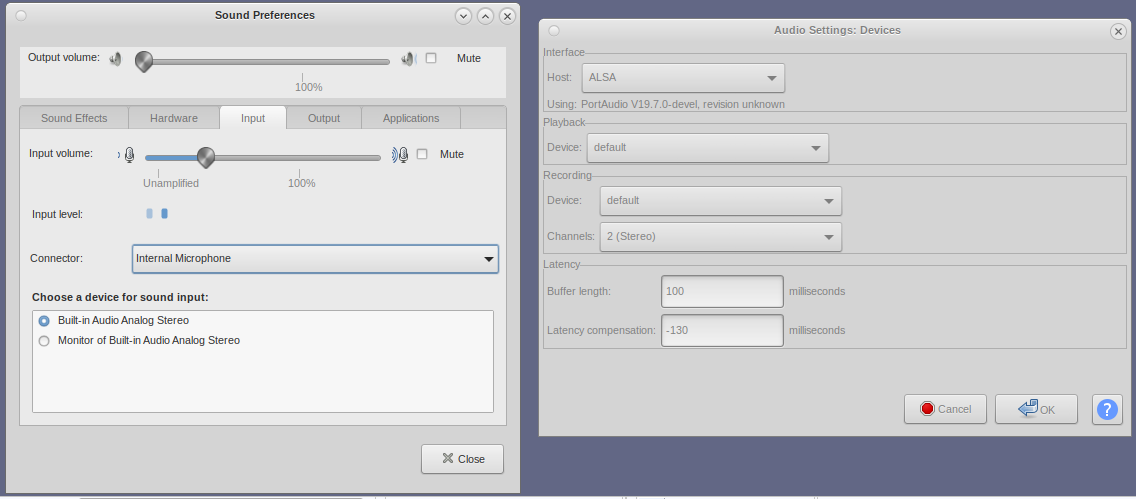
\includegraphics[width=\textwidth]{images/audacity_in_linux}
				\caption{ALSA/PulseAudio di GNU/Linux}
			\end{subfigure}
			\begin{subfigure}[]{.35\textwidth}
				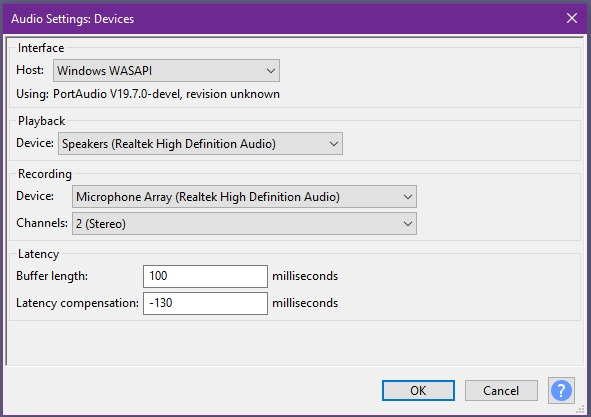
\includegraphics[width=\textwidth]{images/audacity_in_windows}
				\caption{WASAPI di Windows}
			\end{subfigure}
			\caption{Audio Input}
		\end{figure}
	
		\item Jalankan Real-Time Analyzer dan jalankan Signal Generator.
		Pilih White Noise pada volume penuh. Klik Start.
		
		\begin{figure}[H]
			\centering
			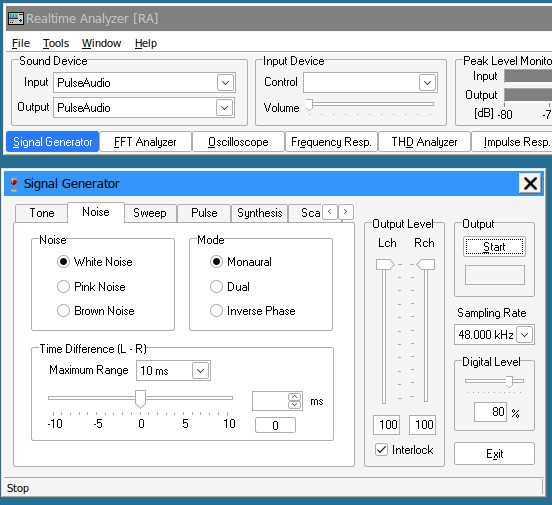
\includegraphics[width=0.6\textwidth,angle=0]{images/rta_noise_gen}
			\caption{Menghasilkan noise}
		\end{figure}
		
		\item Atur Amplifier hingga baca stabil pada nilai tertentu (semisal 81 dB-SPL) pada Sound Level Meter.
		Kemudian rekam noise ruangan di Audacity.
		
		\begin{figure}[H]
			\centering
			\begin{subfigure}[]{.8\textwidth}
				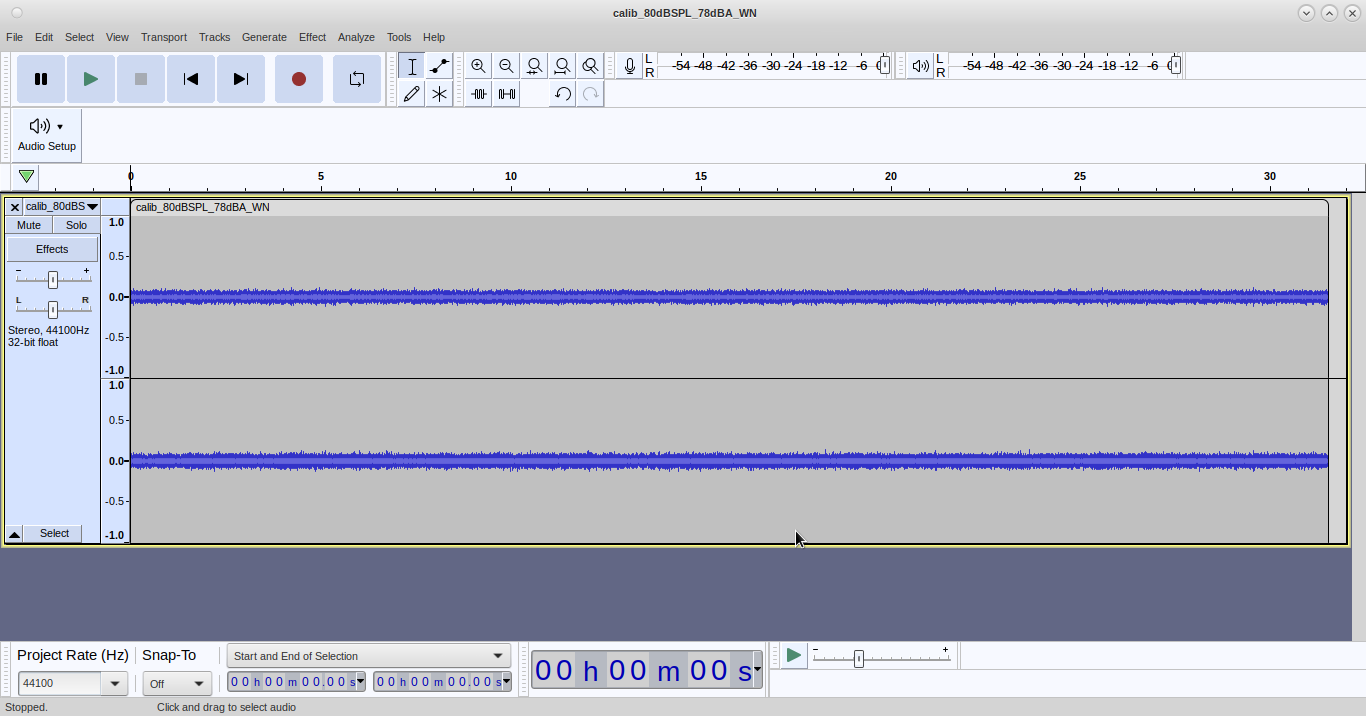
\includegraphics[width=\textwidth]{images/audacity_record}
				\caption{Perekaman di Audacity}
			\end{subfigure}
			\\
			\begin{subfigure}[]{.5\textwidth}
				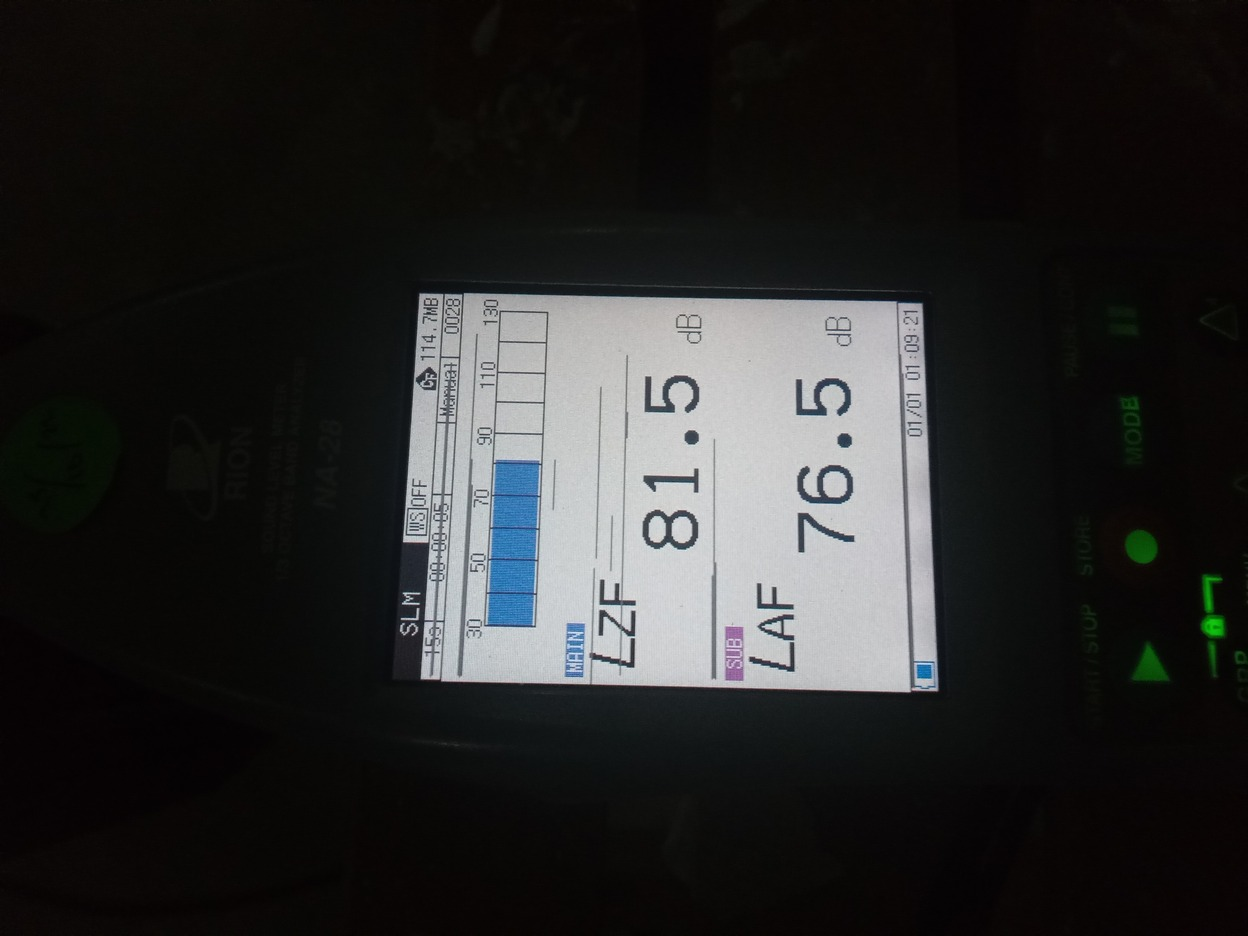
\includegraphics[width=\textwidth]{images/3dio_slm_whitenoise}
				\caption{Nilai terbaca pada SLM}
			\end{subfigure}
			\caption{Perekaman Noise}
		\end{figure}
		
		\item Simpan rekaman dalam format WAV.
		Nama file rekaman memiliki informasi nilai pembacaan SLM.
		
		\item Ulangi langkah di atas untuk Pink Noise.
		
		\begin{figure}[H]
			\centering
			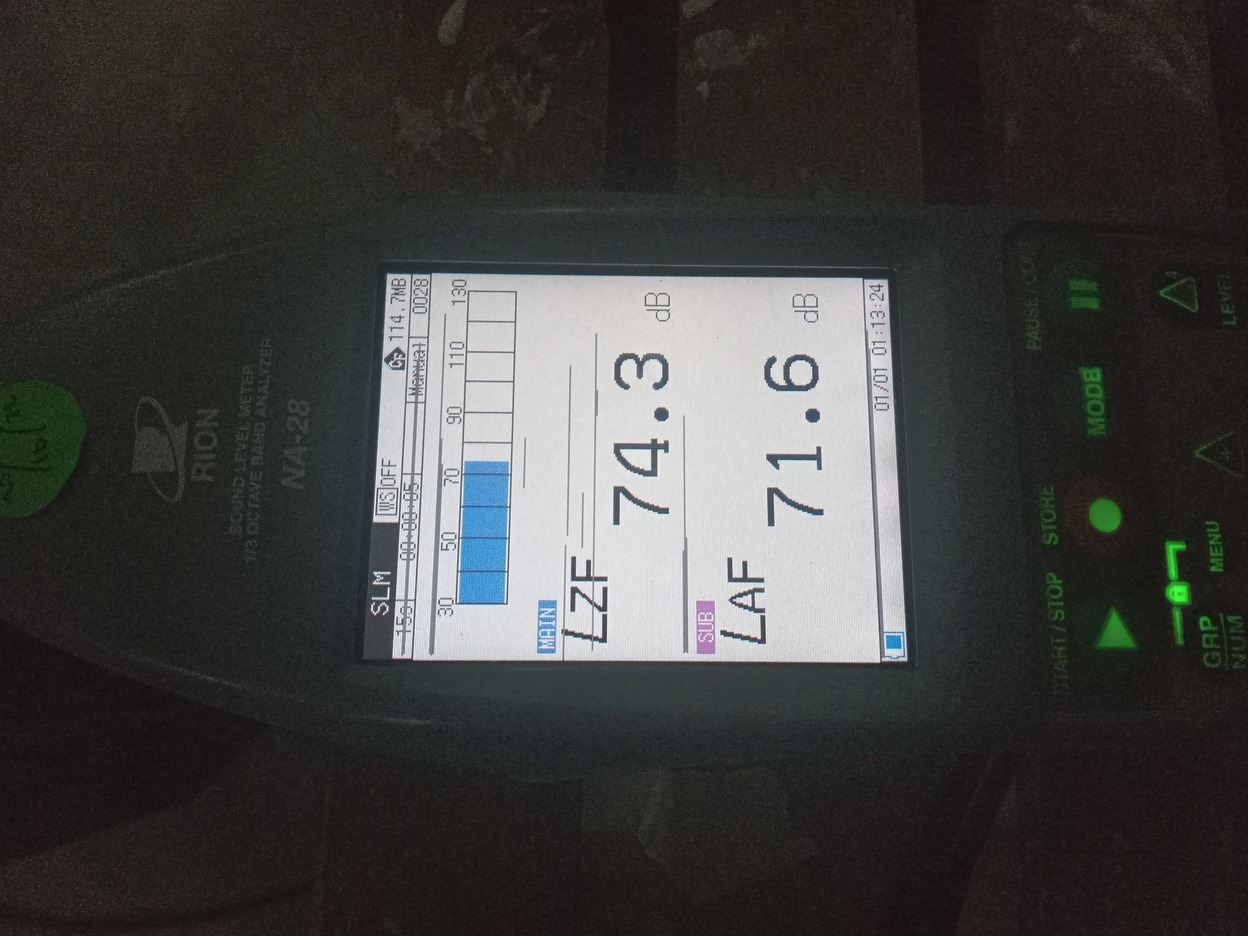
\includegraphics[width=0.5\textwidth,angle=0]{images/3dio_slm_pinknoise}
			\caption{Pembacaan Pink Noise}
		\end{figure}
	\end{itemize}

	\subsubsection{Kalibrasi}
	
	Untuk kalibrasi, kurang lebih juga sama dengan unit EARS sebelumnya.
	Berikut langkah yang dapat dilakukan:
	
	\begin{itemize}
		\item Jalankan Real-Time Analyzer dan buka tab Recorder.
		Pastikan Input adalah PulseAudio (untuk GNU/Linux) atau langsung AudioBox USB 96 (Untuk Windows).
		Kemudian Load rekaman.
		
		\begin{figure}[H]
			\centering
			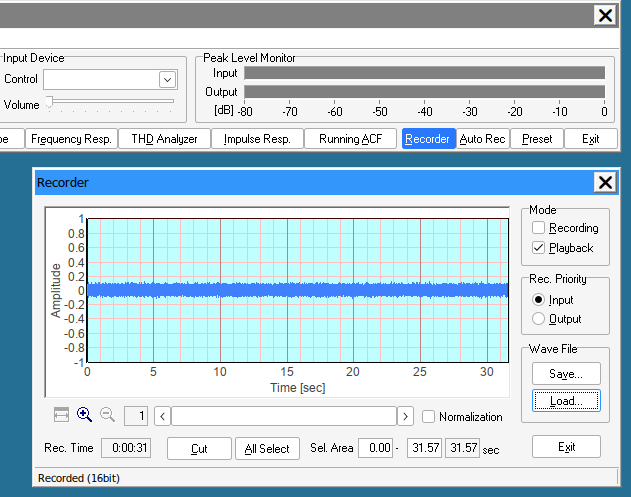
\includegraphics[width=0.6\textwidth,angle=0]{images/rta_load}
			\caption{Loading rekaman ke RTA}
		\end{figure}
		
		Biarkan tab rekaman terbuka.
		
		\item Buka tab FFT Analyzer dan Tekan Calibrate.
		Pilih mode Separate dan atur setiap slider ke nilai 81 dB-SPL sesuai yang terbaca SLM.
		
		\begin{figure}[H]
			\centering
			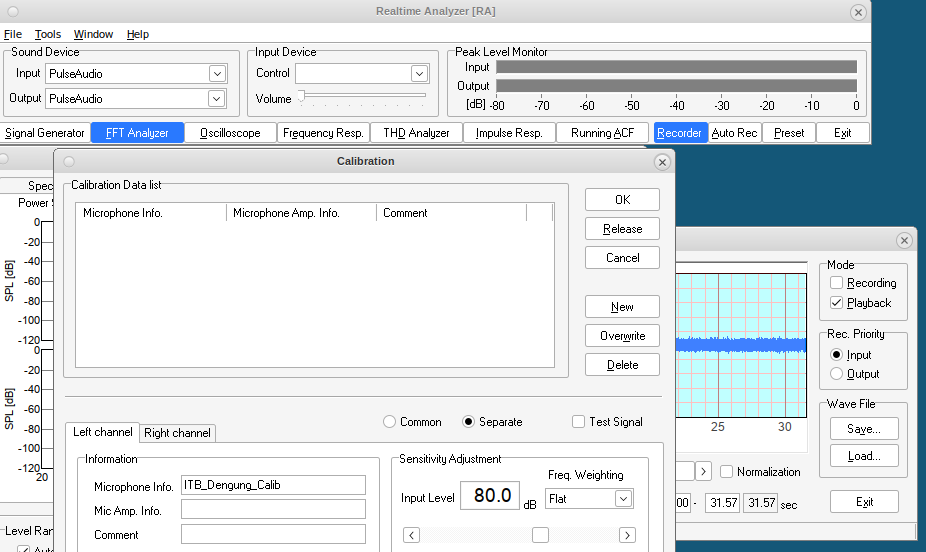
\includegraphics[width=0.8\textwidth,angle=0]{images/rta_calib}
			\caption{Kalibrasi FFT Analyzer}
		\end{figure}
		
		\newpage
		\item Tutup jendela Recorder dan FFT Analyzer terkalibrasi.
		
		\begin{figure}[H]
			\centering
			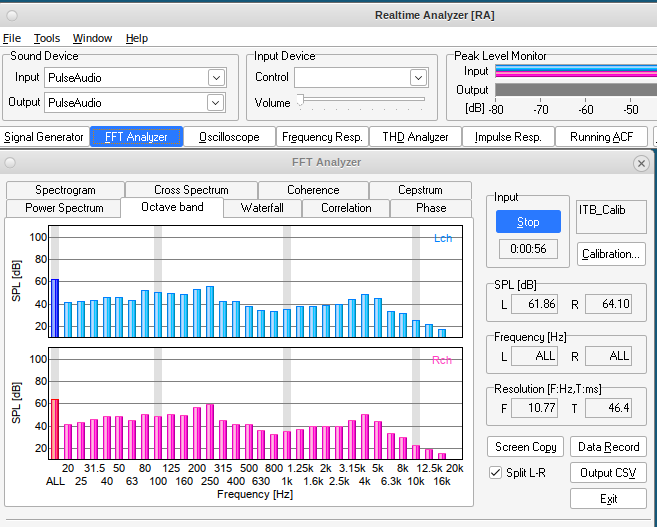
\includegraphics[width=0.8\textwidth,angle=0]{images/rta_fft}
			\caption{Kalibrasi selesai}
		\end{figure}
		
	\end{itemize}

	\newpage
	\subsection{KEMAR}
	
	Berikut rangkuman kegiatan kalibrasi untuk unit Microphone 3DIO.
	
	\subsubsection{Setup}
	
	Berikut setup kalibrasi:
	
	\begin{figure}[H]
		\centering
		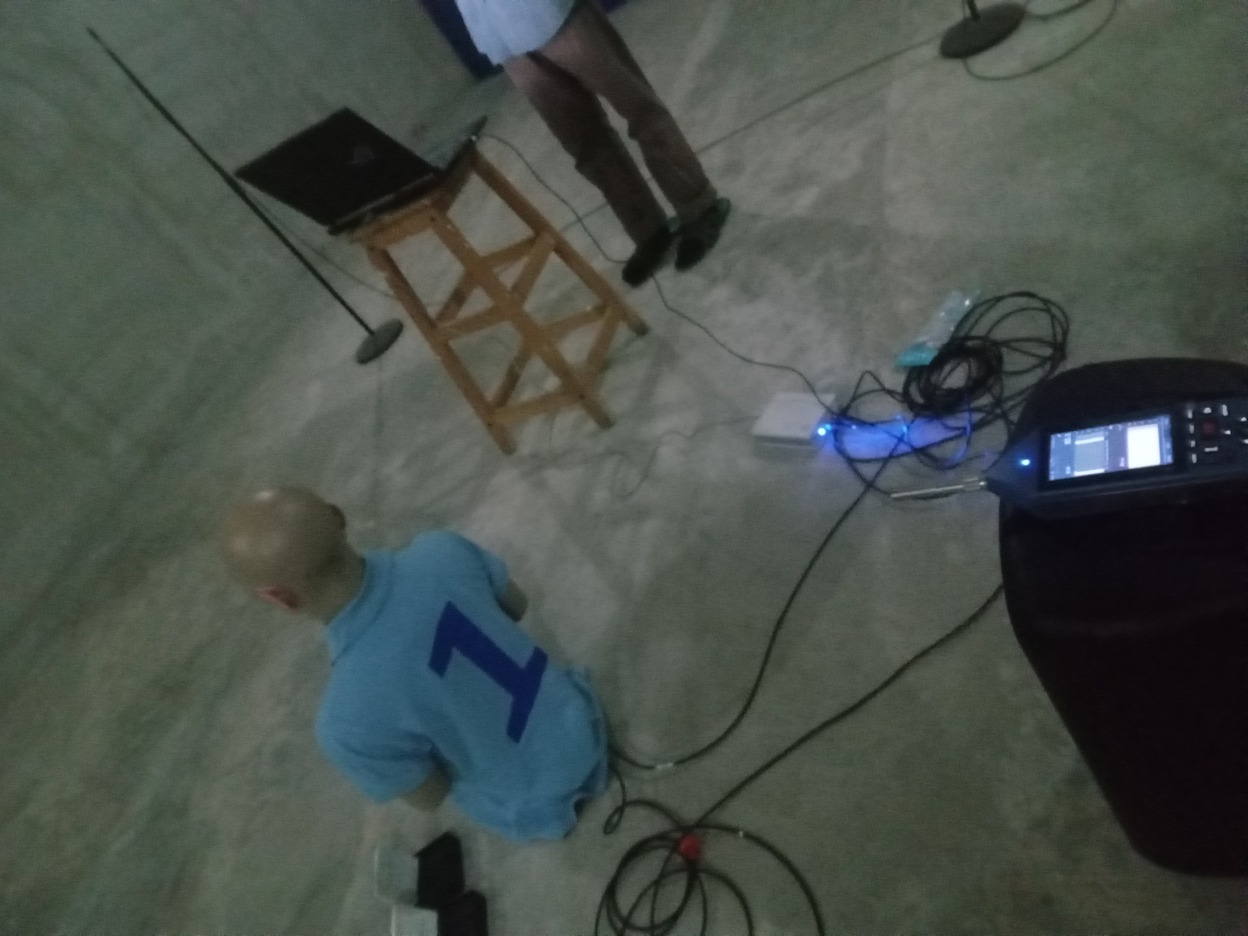
\includegraphics[width=0.75\textwidth,angle=0]{images/kemar_calib_setup}
		\caption{Setup posisi KEMAR, audiobox BSWA, dan Speaker}
	\end{figure}

	\subsubsection{Recording}
	
	Kurang lebih sama dengan unit 3DIO sebelumnya.
	
	\subsubsection{Kalibrasi}
	
	Kurang lebih sama dengan unit 3DIO sebelumnya.
	
	\newpage
	\subsection{Rekaman}
	
	Berkas WAV rekaman dapat di-download di alamat berikut: \href{https://drive.google.com/drive/folders/18bjBI3CSgyAX_4-f_cD2AvmgAtwJ-hkF}{Google-Drive}

	\subsection{Tes Ruang Kedap}
	
	Untuk memastikan hasil kalibrasi, digunakan pengujian pembacaan di ruang kedap.
	Berikut setup pengujian di Ruang Kedap:
	
	\begin{figure}[H]
		\centering
		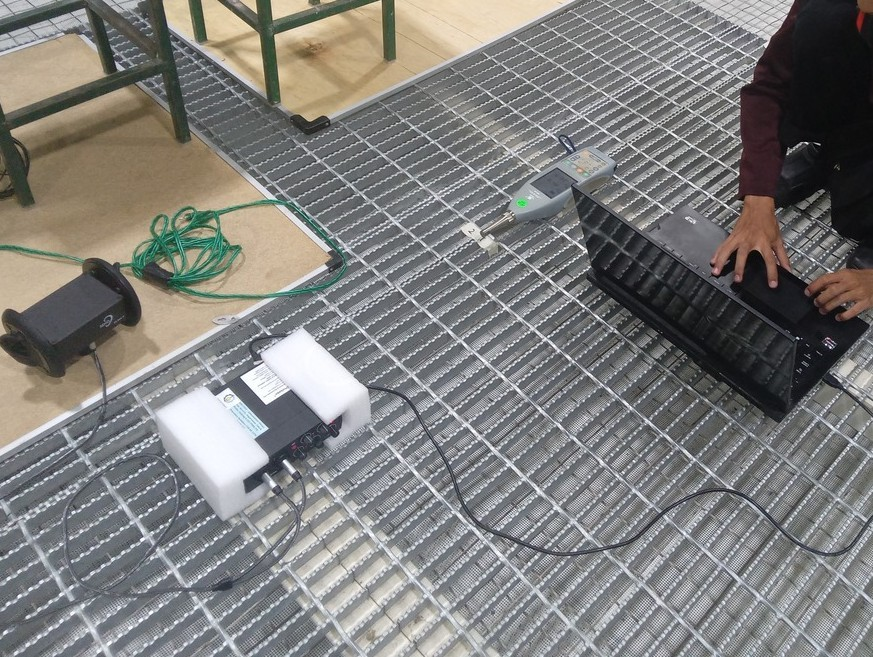
\includegraphics[width=0.6\textwidth,angle=0]{images/tes_kedap}
		\caption{Setup Uji di ruang Kedap}
	\end{figure}
	
	Hasilnya ada selisih kisaran 6dB-SPL antara pembacaan SLM dan unit 3DIO yang terbaca di software RTA.
	
	\begin{figure}[H]
		\centering
		\begin{subfigure}[]{.45\textwidth}
			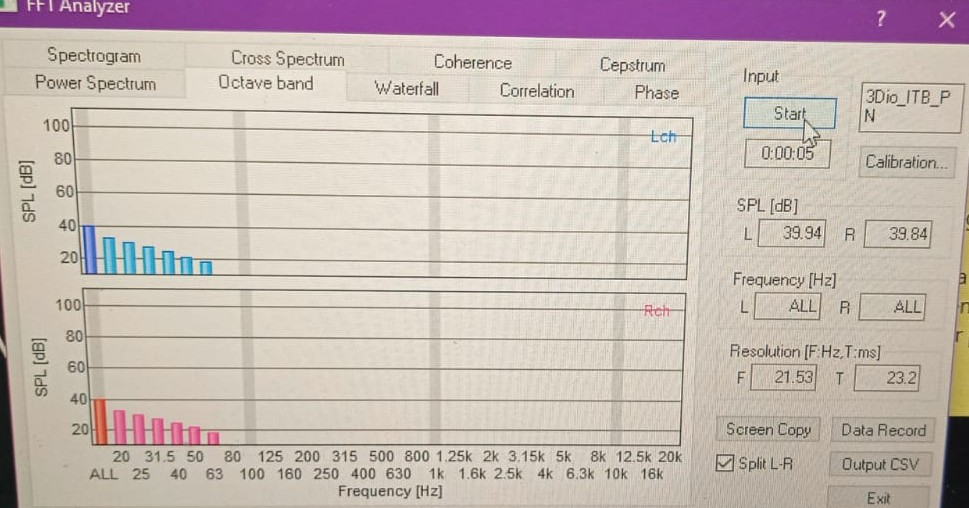
\includegraphics[width=\textwidth]{images/tes_kedap_rta}
			\caption{Nilai RTA dari 3DIO}
		\end{subfigure}
		\\
		\begin{subfigure}[]{.45\textwidth}
			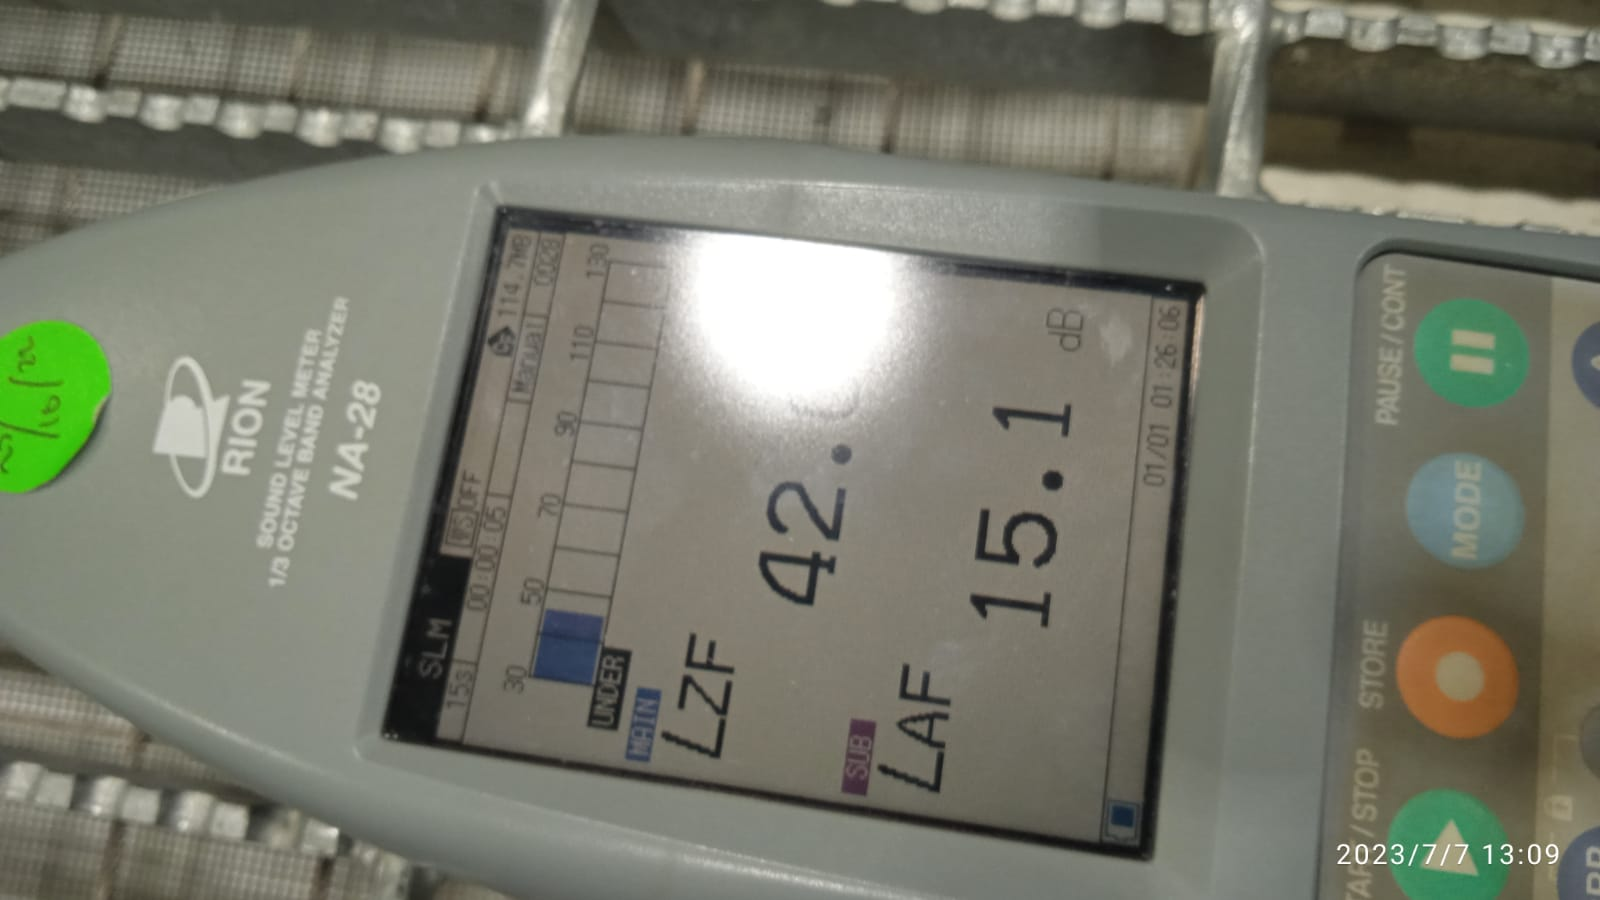
\includegraphics[width=\textwidth]{images/tes_kedap_slm}
			\caption{Nilai SLM}
		\end{subfigure}
		\caption{Tes pada Ruang Kedap}
	\end{figure}

	Secara umum memang ada perbedaan nilai sekitar 10dB-SPL antara pengukuran SLM dan dummy head seperti perangkat 3DIO\cite{Sudarsono2018}.
	
	\newpage
	\section{Daftar Pustaka}
	
	\bibliographystyle{IEEEtran}
	\bibliography{/home/achmaday/Documents/library.bib}

\end{document}
